\documentclass{./plantilla/umss}

\usepackage[dvipsnames]{xcolor}
\definecolor{bg}{rgb}{0.95,0.95,0.95}

\usepackage{booktabs}
\usepackage{array}
\usepackage{multirow}
\usepackage{enumitem}
\usepackage{minted}
\usepackage{listings}
\usepackage{pdfpages}

\setminted{
  fontsize=\small,
  linenos=true,
  breaklines=true,
  frame=lines,
  framesep=2mm,
  bgcolor=gray!10
}

\title{Informe grupal}

\begin{document}

\sujet{Red Social - Grupo DuckCoders}
\enseignant{Ing. Rosemary \textsc{Torrico}}
\eleves{\begin{small}

  \begin{itemize}
    \item Alfredo Ronald Choquerive Toroya
    \item Nicole Geraldine Rodas Cornejo
    \item Valentina Mercado Apaza
    \item Franco Prieto Ayala
    \item Adriana Lavayen Iguay
    \item Shamir Leonardo Terán Mustafá
    \item Angelica Adriana Soto Jiménez
    \item Jhosua Alejandro Bustillos Calderon
    \item Brenda Vargas Mollo
    \item Pablo Adrian Azurduy Rivera
  \end{itemize}
\end{small}}

\fairemarges
\fairepagedegarde

\section{Resumen de la película The Social Network}

La película narra El comienzo de Facebook (actualmente Meta), centrada en la figura de Mark Zuckerberg, un estudiante de Harvard que, tras ser rechazado socialmente, crea inicialmente \textit{Facemash} y posteriormente \textit{TheFacebook}. La trama entrelaza la evolución técnica de la plataforma con las complejas batallas legales contra los gemelos Winklevoss y su socio fundador y primer inversor, Eduardo Saverin. 

A través de una narrativa no lineal que alterna el presente de los litigios con el pasado de la creación, se expone cómo la ambición desmedida de Zuckerberg y la visión empresarial de Sean Parker transformaron un proyecto universitario en un imperio global. La historia destaca no solo el auge tecnológico, sino el costo humano del éxito: la sistemática destrucción de los vínculos personales de Zuckerberg en su ascenso hacia la cima del mundo digital.

\section{Opiniones Personales}

\begin{itemize}
  \item \textbf{El comienzo tóxico y la validación personal:} 
        Resulta inquietante cómo la película expone que Facebook no nació de un ideal altruista de ``conectar al mundo'', sino del resentimiento y el morbo. La raíz del proyecto se encuentra en \textit{Facemash} (la cosificación de las mujeres) y en el despecho tras una ruptura sentimental. Zuckerberg no buscaba inicialmente revolucionar las comunicaciones, sino obtener validación, estatus y pertenencia a élites que lo rechazaban. Esto humaniza al villano, pero a la vez revela la naturaleza narcisista sobre la que se cimentó la red social más grande del planeta.

  \item \textbf{La arquitectura presente en la pelicula:} 
        Desde una perspectiva técnica, la cinta ilustra magistralmente la transición crítica de un \textit{script} universitario a un sistema distribuido escalable. Lo más valioso es ver cómo los problemas de ingeniería dejan de ser sintácticos para convertirse en desafíos de arquitectura, mantenimiento y adaptación a una demanda exponencial. La película enseña que el éxito en el desarrollo de software no depende solo de la capacidad de codificar (como hacía Mark en su dormitorio), sino de la visión para estructurar un producto que pueda sostener el crecimiento y las nuevas necesidades del negocio.

  \item \textbf{La idea y la Ejecucion de esta:} 
        El conflicto con los gemelos Winklevoss y Eduardo Saverin resalta una lección brutal del emprendimiento tecnológico: la idea por sí sola no tiene valor; la ejecución lo es todo. Mientras los demás se obsesionaban con la propiedad intelectual y el crédito, Zuckerberg entendió que la velocidad de implementación y la adaptabilidad del producto eran superiores a cualquier contrato o idea original. La película cuestiona la moralidad de este proceso, pero confirma que en la industria digital, la historia la escriben quienes construyen, no quienes imaginan.

  \item \textbf{La paradoja del genio asocial:} 
        El personaje de Zuckerberg encarna la contradicción suprema, es un visionario capaz de conectar a millones de personas, pero es incapaz de mantener una conexión empática con su entorno inmediato. Su genialidad técnica contrasta con su torpeza emocional, lo que sugiere que la red social fue un mecanismo de compensación. Al final, logra el poder y el reconocimiento que buscaba, pero termina aislado, demostrando que la herramienta que creó para unir a otros, terminó por desconectarlo a él de la realidad humana.

  \item \textbf{La ambición como motor destructivo en las relaciones:} 
        La evolución de Mark, influenciada por la figura de Sean Parker, muestra cómo la ética se flexibiliza en pos del crecimiento exponencial. La traición a Eduardo Saverin no se presenta solo como un acto de maldad, sino como una ``necesidad'' fría para la supervivencia de la empresa bajo la lógica del capital de riesgo. La película deja la reflexión de que las oportunidades que Mark aprovechó, aunque moralmente cuestionables, fueron los cimientos pragmáticos de lo que hoy es Meta; un recordatorio de que la historia tecnológica a menudo se escribe con tinta de lealtades rotas.
\end{itemize}



\newpage
\section{Imagenes del grupo}

\begin{center}
  
\includegraphics[width=0.60\textwidth]{images/primer1.jpeg}
\end{center}

\begin{center}
  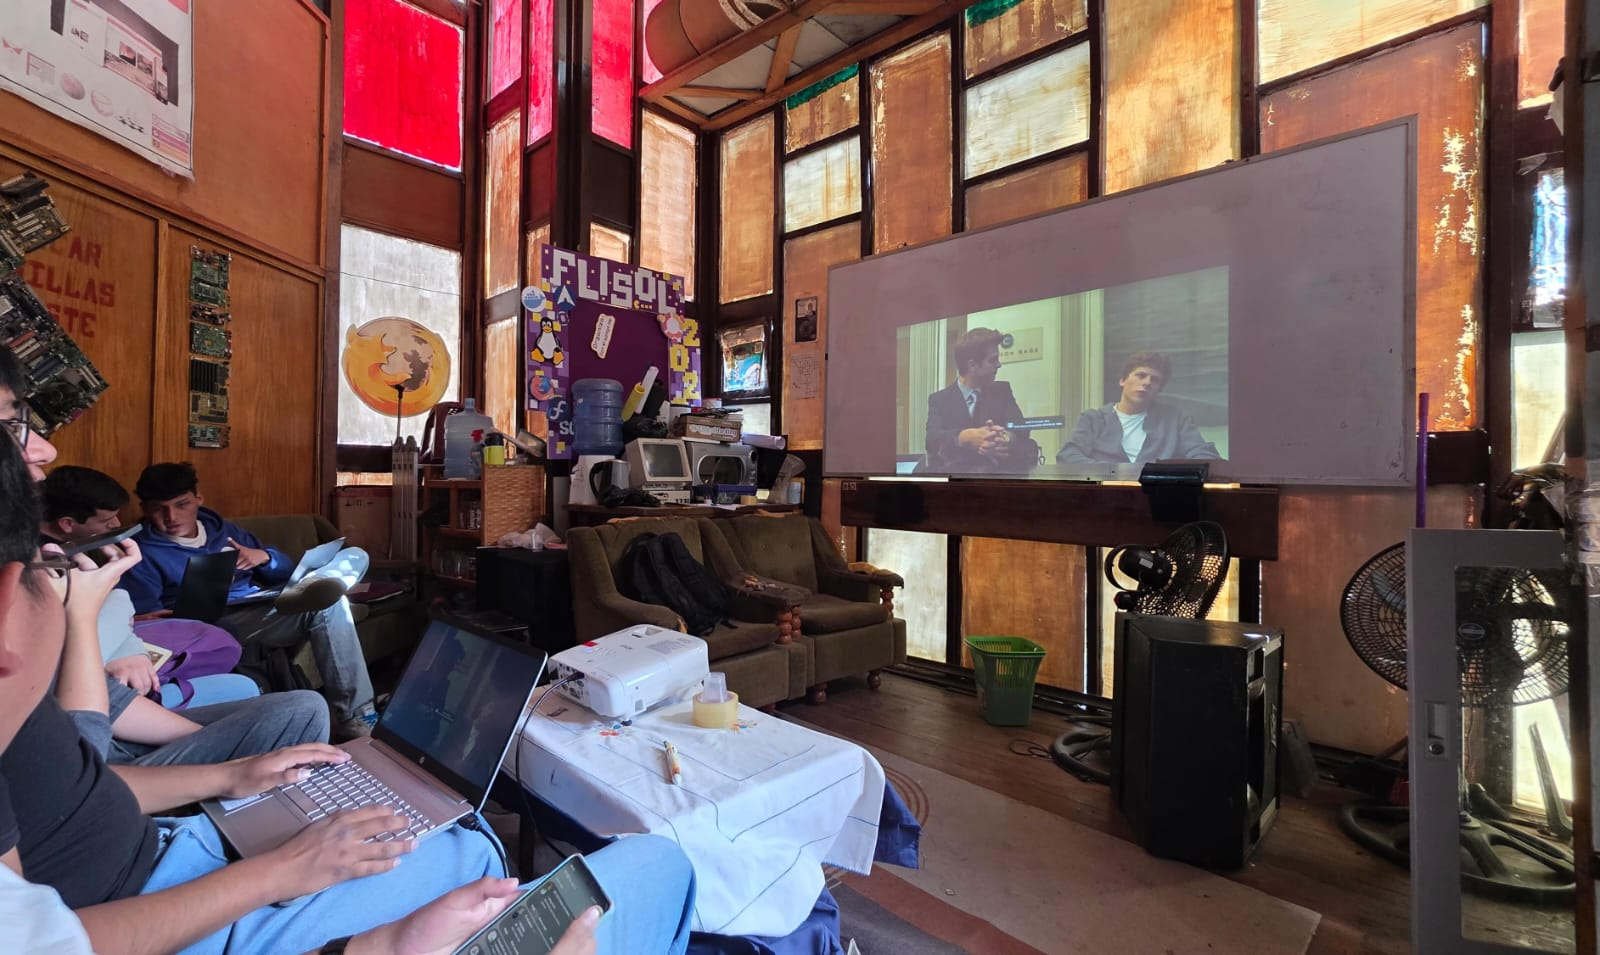
\includegraphics[width=0.60\textwidth]{images/primer2.jpeg}
\end{center}

\begin{center}
  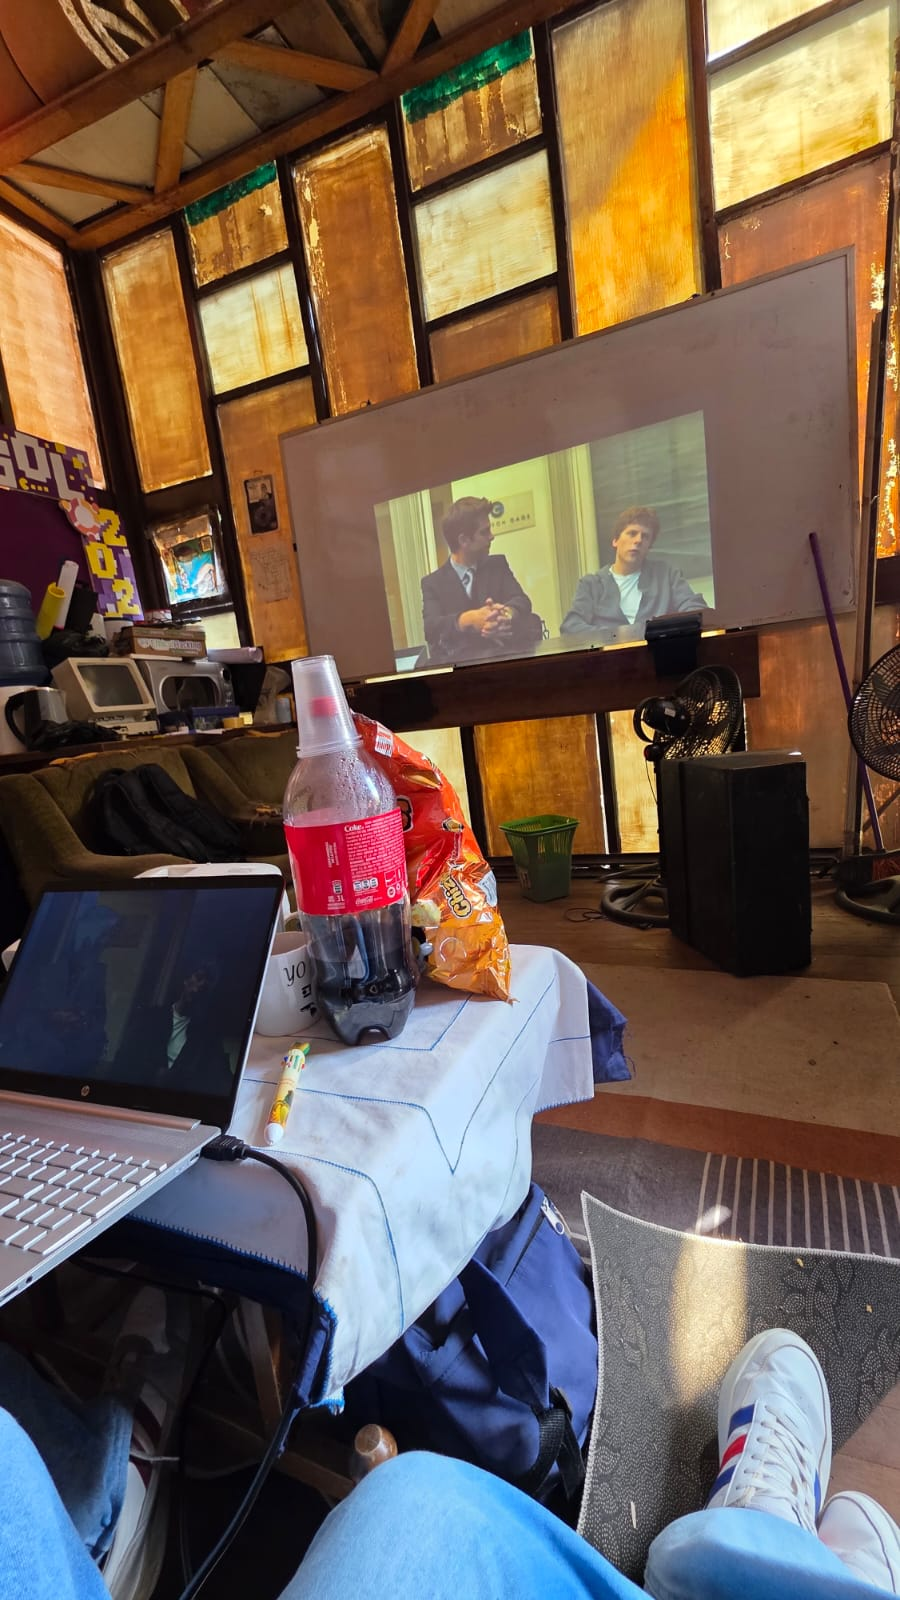
\includegraphics[width=0.30\textwidth]{images/primer3.jpeg}
\end{center}

\end{document}
